\documentclass[10pt,a4paper,spanish]{article}

\usepackage[T1]{fontenc} 
\usepackage[utf8]{inputenc}
\usepackage[spanish]{babel}

\usepackage{graphicx}
\usepackage{epstopdf}

\usepackage[export]{adjustbox}
\usepackage{caption}
\usepackage{colortbl} 
\usepackage{dashrule} 
\usepackage{fancyhdr}
\usepackage{float}
\usepackage{framed}
\usepackage[bmargin=2cm,footnotesep=1cm,tmargin=2cm]{geometry} 
\usepackage[pdftex,colorlinks,backref,bookmarks=true,bookmarksnumbered=true,linkcolor=black,urlcolor=black,citecolor=black]{hyperref}
\usepackage[section]{placeins}
\usepackage[labelsep=quad,indention=10pt]{subfig}
\usepackage[spanish,shadow,textsize=small]{todonotes}
\usepackage{wrapfig}

% TITULOS
\newcommand{\asig}{Algoritmos y Estructuras de Datos}
\newcommand{\anno}{3º}
\newcommand{\grado}{Grado en Ingeniería Biomédica}
\newcommand{\upm}{Universidad Politécnica de Madrid}
\newcommand{\curso}{}
\newcommand{\ssg}{Rodrigo García Carmona}
\newcommand{\email}{\href{mailto:rodrigo.garciacarmona@ceu.es}{rodrigo.garcia@upm.es}}
\newcommand{\cabecera}[1]{
  \title{Guion de Prácticas}
  \author{\asig\\ \anno\grado\\ \ceu \\ \ssg} 
  \date{#1}
  \maketitle \thispagestyle{fancy}
}

% NUEVAS TODONOTES
\newcommand{\nota}[2][] {\todo[inline, #1]{#2}}
\newcommand{\corregir}[2][] {\todo[color=red, #1]{#2}}
\newcommand{\finaltodo}[2][] {\todo[color=green!40,fancyline #1]{#2}}
\newcommand{\finalnota}[2][] {\todo[color=green!40, inline #1]{#2}}

% PDF
\hypersetup{
  colorlinks=true,
  linkcolor=blue,
  filecolor=magenta,      
  urlcolor=cyan,
  pdfauthor={\ssg},
  pdftitle={Guion de Prácticas},
  pdfsubject={\asig, \grado, \upm, Madrid, España},
  pdfkeywords={algoritmos, estructuras de datos, ingeniería biomédica, guion, prácticas}, 
  pdftoolbar=true,
  pdfmenubar=true,
  pdffitwindow=true,
  pdfnewwindow=true
}

% ENCABEZADO
\pagestyle{fancy}%
  \renewcommand{\headrulewidth}{0.1pt}
  \renewcommand{\footrulewidth}{0.1pt}
  \fancyhf{}
  \fancyhead[L]{
\includegraphics[width=8mm]{templates/ETSIT-UPM.eps}}
  \fancyhead[C]{\small{\asig}\\\small{\grado}}
  \fancyhead[R]{\curso}
  \fancyfoot[L]{}
  \fancyfoot[C]{\thepage}
  \fancyfoot[R]{}

% CAJA SOMBREADA
% comando \sombreado{Título}{Texto}
\definecolor{shadecolor}{rgb}{0.9,0.9,0.9}
\newcommand{\sombreado}[2]{
  \begin{shaded}
    \begin{center} \emph{\textsc{#1}} \end{center}
    \noindent #2\\
  \end{shaded}
}

% CAJA INSTRUCCIONES 
\definecolor{shadecolor}{rgb}{0.9,0.9,0.9}
\newcommand{\instrucciones}[7]{
  \begin{shaded}
    \begin{center} \emph{\textsc{#1}}
    \end{center}
    %\noindent \emph{\textsc{Fecha límite de entrega: }} \emph{#4}\\
    %\emph{\textsc{Peso: }}\emph{#5}\newline\newline
    #6

    #7
  \end{shaded}
}

% Código fuente
\newcommand{\code}[1]{\texttt{#1}}

% Minted
\usepackage{minted}
% Optional: Set a default style. 'manni' is a light, clean style.
% Other popular styles include 'tango', 'monokai', 'solarized-light'.
\usemintedstyle{sas}

% PRACTICA
\newcommand{\practica}{Práctica 1: Repaso de Java}
\newcommand{\notaob}{
\begin{center}
Rodrigo García Carmona\footnotemark\\
\href{mailto:rodrigo.garcia@upm.es}{rodrigo.garcia@upm.es}\\
\includegraphics[width=20mm]{templates/by-nc-sa.eps}
\end{center}

Esta práctica es individual y sirve tanto para desarrollar como para poner a prueba los conocimientos adquiridos. Realizar esta práctica es recomendable para aumentar las probabilidades de éxito en los exámenes teóricos.
}

% MACROS

% CONTENIDO
\begin{document}

\instrucciones{\practica}{\tiempo}{\obligatoria}{\fecha}{\peso}{\notaob}

\section{Preparación de la práctica}
\footnotetext{Desarrollada a partir del trabajo previo de Miguel Ángel de Miguel.}

El objetivo de esta práctica es refrescar los conocimientos de Java, ya que, en condiciones ideales, hará dos años que superó la asignatura Fundamentos de Programación de primer curso. En esta práctica repasará los siguientes conceptos:

\begin{itemize}
    \item Uso de tipos de datos primitivos, arrays, objetos y colecciones.
    \item Uso de sentencias de control de flujo.
    \item Creación de algoritmos sencillos.
    \item Lectura y escritura de archivos.
    \item Implementación de interfaces y estructuración de proyectos \textit{software}.
\end{itemize}

\sombreado{Trabajo previo al laboratorio}{El tiempo de las clases de laboratorio es muy valioso, ya que en ellas tendrá a su disposición a los profesores para resolver cualquier duda que le pueda surgir. Por tanto, para facilitar al máximo el aprovechamiento de este tiempo, las prácticas se han dividido en varias secciones. La primera de ellas (``preparación de la práctica'') puede ¡y debe! realizarse \textbf{antes de la sesión de laboratorio} propiamente dicha. Leer esta sección antes de entrar a clase hará que su tiempo en el laboratorio sea más productivo y provocará que las dudas más importantes le surjan \textbf{durante la clase}, y \textbf{no después}, cuando se encuentre estudiando solo en su casa y la única opción que le quede sea escribir un email al profesor.

De hecho, es especialmente importante evitar que se den situaciones como esta la noche antes de un examen.}

\subsection{OpenBCI}

Los BCI (\textit{Brain Computer Interfaces}, interfaces cerebro-ordenador) son dispositivos que permiten interactuar con un ordenador a través de las señales eléctricas que produce el cerebro humano, las mismas que forman la base del pensamiento. Esto hace posible, usando un lenguaje coloquial, ``controlar un ordenador con la mente''.

Existe una gran variedad de dispositivos BCI, que se pueden clasificar, a grandes rasgos, en invasivos y no invasivos. Los invasivos se introducen directamente en contacto con el cerebro de una persona (o animal), mientras que los no invasivos no precisan de ninguna operación quirúrgica o incisión. Lógicamente, los primeros permiten acceder a las señales eléctricas del cerebro de forma directa y obtienen datos de más calidad, pero tienen la contrapartida de que implican la inserción de un objeto extraño en el interior del cuerpo humano, lo que puede ocasionar rechazos, precisar de operaciones constantes (las neuronas se mueven dentro del cerebro) y otros muchos problemas.

Hoy en día, cuando el común de los mortales piensa en dispositivos BCI, lo más probable es que lo primero que le venga a la mente (je) sea Neuralink, la empresa del polémico Elon Musk, que está desarrollando dispositivos invasivos. Pero no es la única que investiga en el campo de los BCI. En el otro extremo se encuentra \href{https://openbci.com/}{OpenBCI}, una empresa pequeña (en comparación con Neuralink) que se financió a través de campañas de \textit{crowdfunding} y que produce dispositivos BCI no invasivos que cualquier persona con los medios necesarios puede construir, pues es un proyecto de código abierto (\textit{open source}) y \textit{hardware} abierto (\textit{open hardware)}.

\sombreado{\textit{Open source} y \textit{open hardware}}{El \textit{open source} es un movimiento (o una filosofía, según a quién pregunte) que promueve que el código fuente de los programas informáticos sea hecho público (``liberado''). Este movimiento afirma que, si uno solo dispone de los programas compilados, sin el código fuente, no es verdadero dueño del \textit{software} que utiliza, ya que no puede modificarlo, mejorarlo o utilizarlo de formas distintas a las que concibió quien se lo vendió. Además, no disponer de este código impide saber qué está haciendo realmente el \textit{software} y nos hace dependientes del fabricante original para obtener soporte o reparaciones. El movimiento \textit{open source} está muy relacionado con otros como el \textit{right to repair} (derecho a reparar), el \textit{maker manifesto} (democratizar la fabricación de dispositivos tecnológicos), la cultura \textit{hacker}, el \textit{open access} (ciencia abierta) o el \textit{open hardware} (\textit{hardware} que viene acompañado de las instrucciones para replicarlo), entre otros.

Si siente curiosidad, investigue estas u otras iniciativas relacionadas. Quizá entregar el acceso y control sobre nuestros pensamientos a una empresa privada que ejecuta \textit{software} cuyo funcionamiento real desconocemos no sea la mejor de las ideas.}

Hasta la fecha, OpenBCI ha creado dos placas, la OpenBCI 32 Bit (ver Figura \ref{fig:openBCI}) y la Ganglion, que cuentan con amplificadores biométricos y que se pueden conectar a electrodos que se colocan sobre la piel para capturar varias señales eléctricas producidas por el cuerpo humano: EMG (electromiograma), ECG (electrocardiograma) y EEG (electroencefalograma).

\begin{figure}[!htbp]
  \centering
  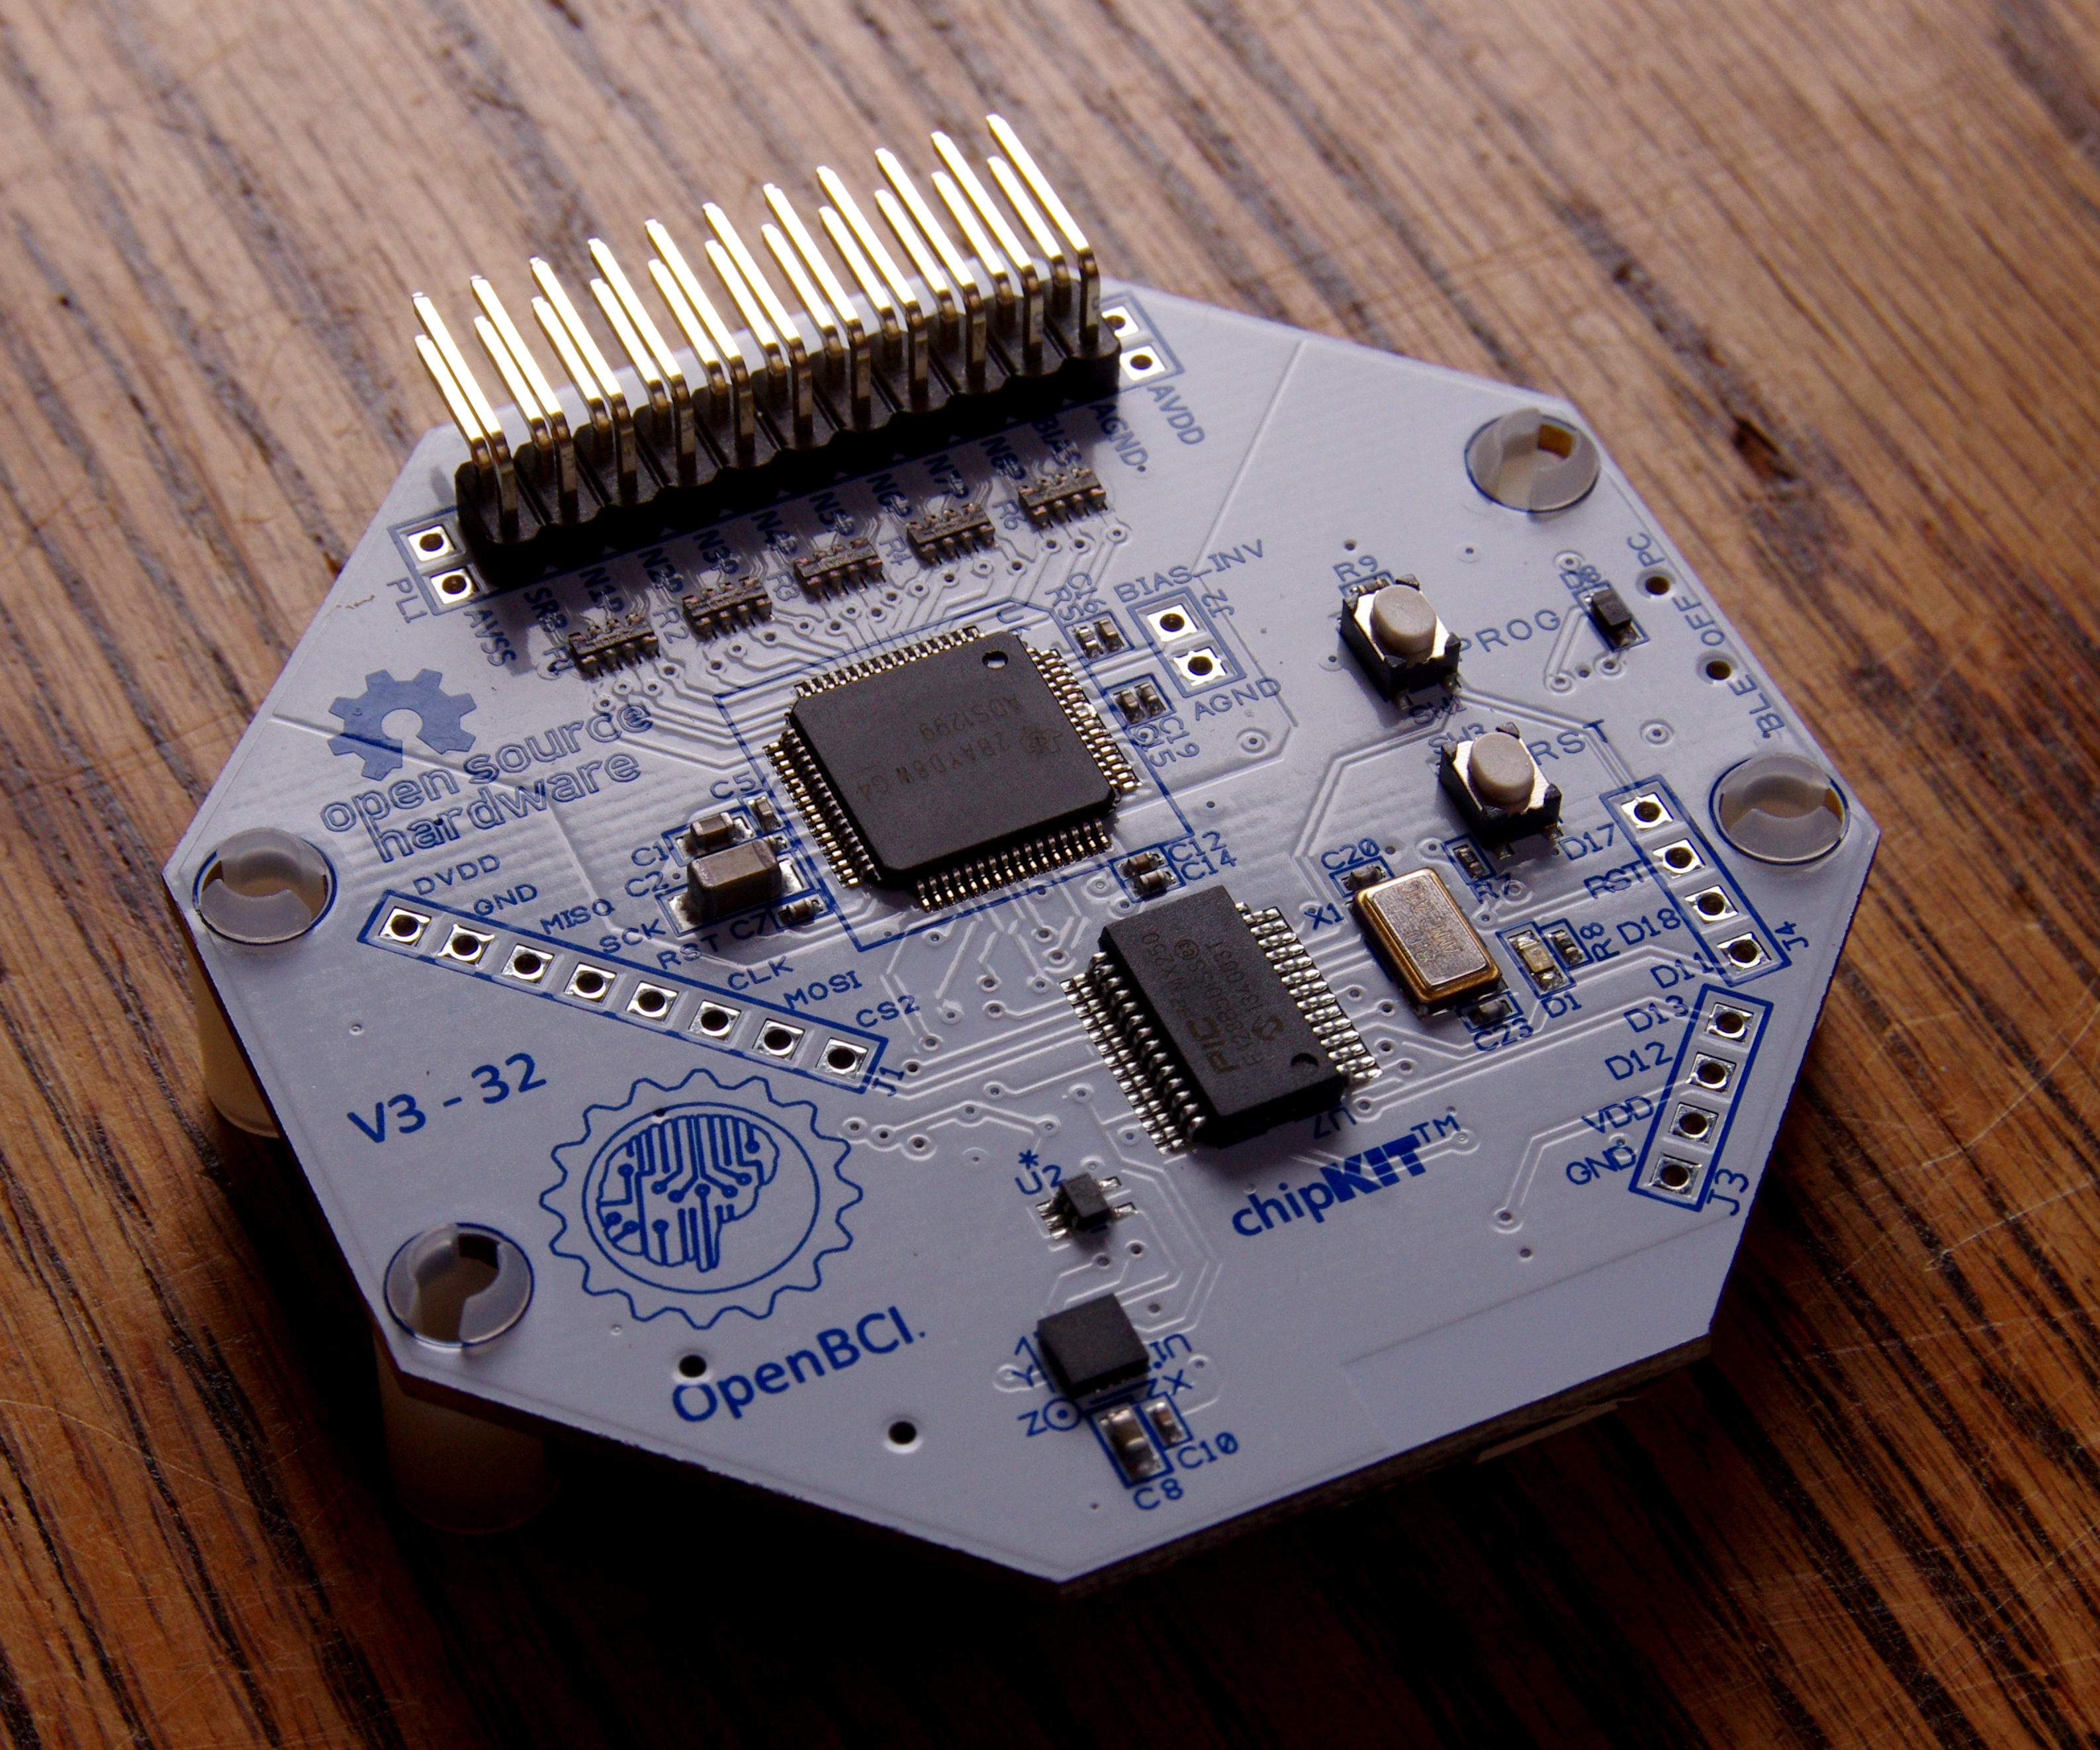
\includegraphics[width=0.8\textwidth]{files/OpenBCI.png}
  \caption{Placa OpenBCI 32 Bit\protect\footnotemark}
  \label{fig:openBCI}
\end{figure}
\footnotetext{\href{https://commons.wikimedia.org/w/index.php?curid=37520130}{Omphalosskeptic - CC BY-SA 4.0}}

Estas señales, una vez capturadas, pueden transmitirse a otros dispositivos a través de protocolos de comunicaciones como Bluetooth, lo que permite integrar los dispositivos que siguen el estándar OpenBCI con, por ejemplo, un \textit{headset} de realidad virtual (ver Figura \ref{fig:varjoXR3}), lo que nos permitiría utilizar estas señales como comandos con los que controlar a un avatar en un entorno virtual. 

\begin{figure}[!htbp]
  \centering
  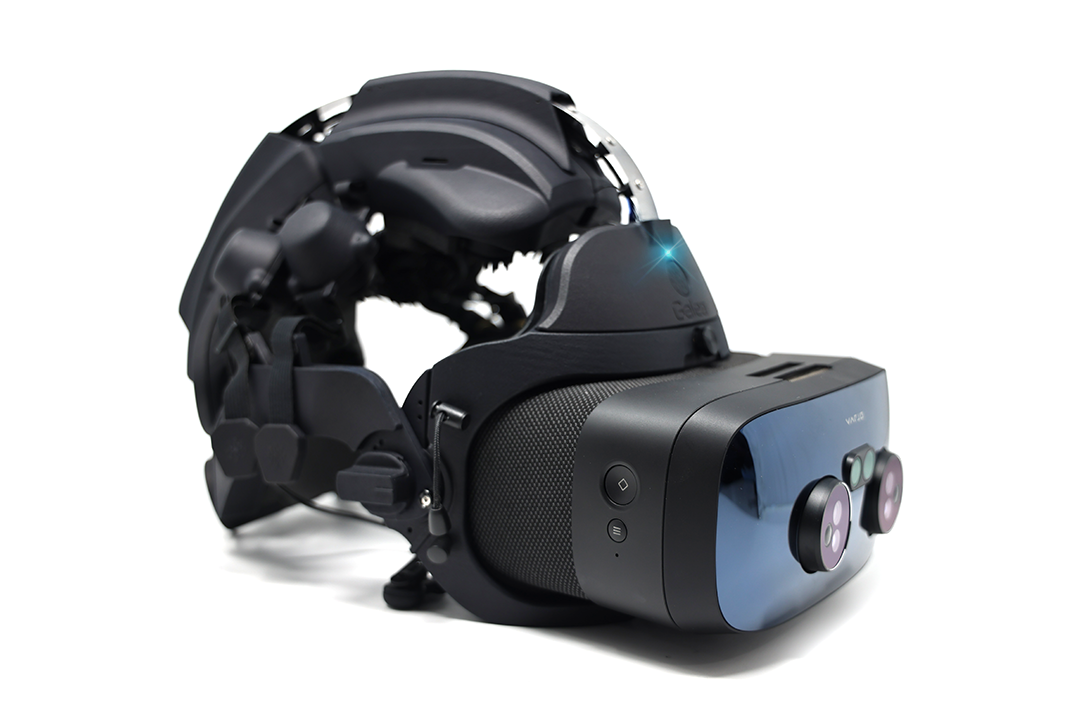
\includegraphics[width=0.8\textwidth]{files/OpenBCI-Galea-Varjo-XR3.png}
  \caption{OpenBCI con el dispositivo de realidad virtual Varjo XR3\protect\footnotemark}
  \label{fig:varjoXR3}
\end{figure}
\footnotetext{\href{https://commons.wikimedia.org/w/index.php?curid=159523578}{Carillons - CC BY-SA 4.0}}

Si dispone de conocimientos de programación y de electrónica, sabe soldar y tiene ganas de cacharrerar, la creación de un entorno como este está a su alcance.

\subsection{Grabaciones de EEG}
\label{eeg}

Para obtener las señales eléctricas del cerebro (EEG) de forma no invasiva se utilizan una serie de electrodos colocados en diferentes partes de la cabeza de una persona, habitualmente dispuestos de una forma concreta gracias a un ``casco'' o ``gorro'' como el que aparece en la Figura \ref{fig:ultracortex}.

\begin{figure}[!htbp]
  \centering
  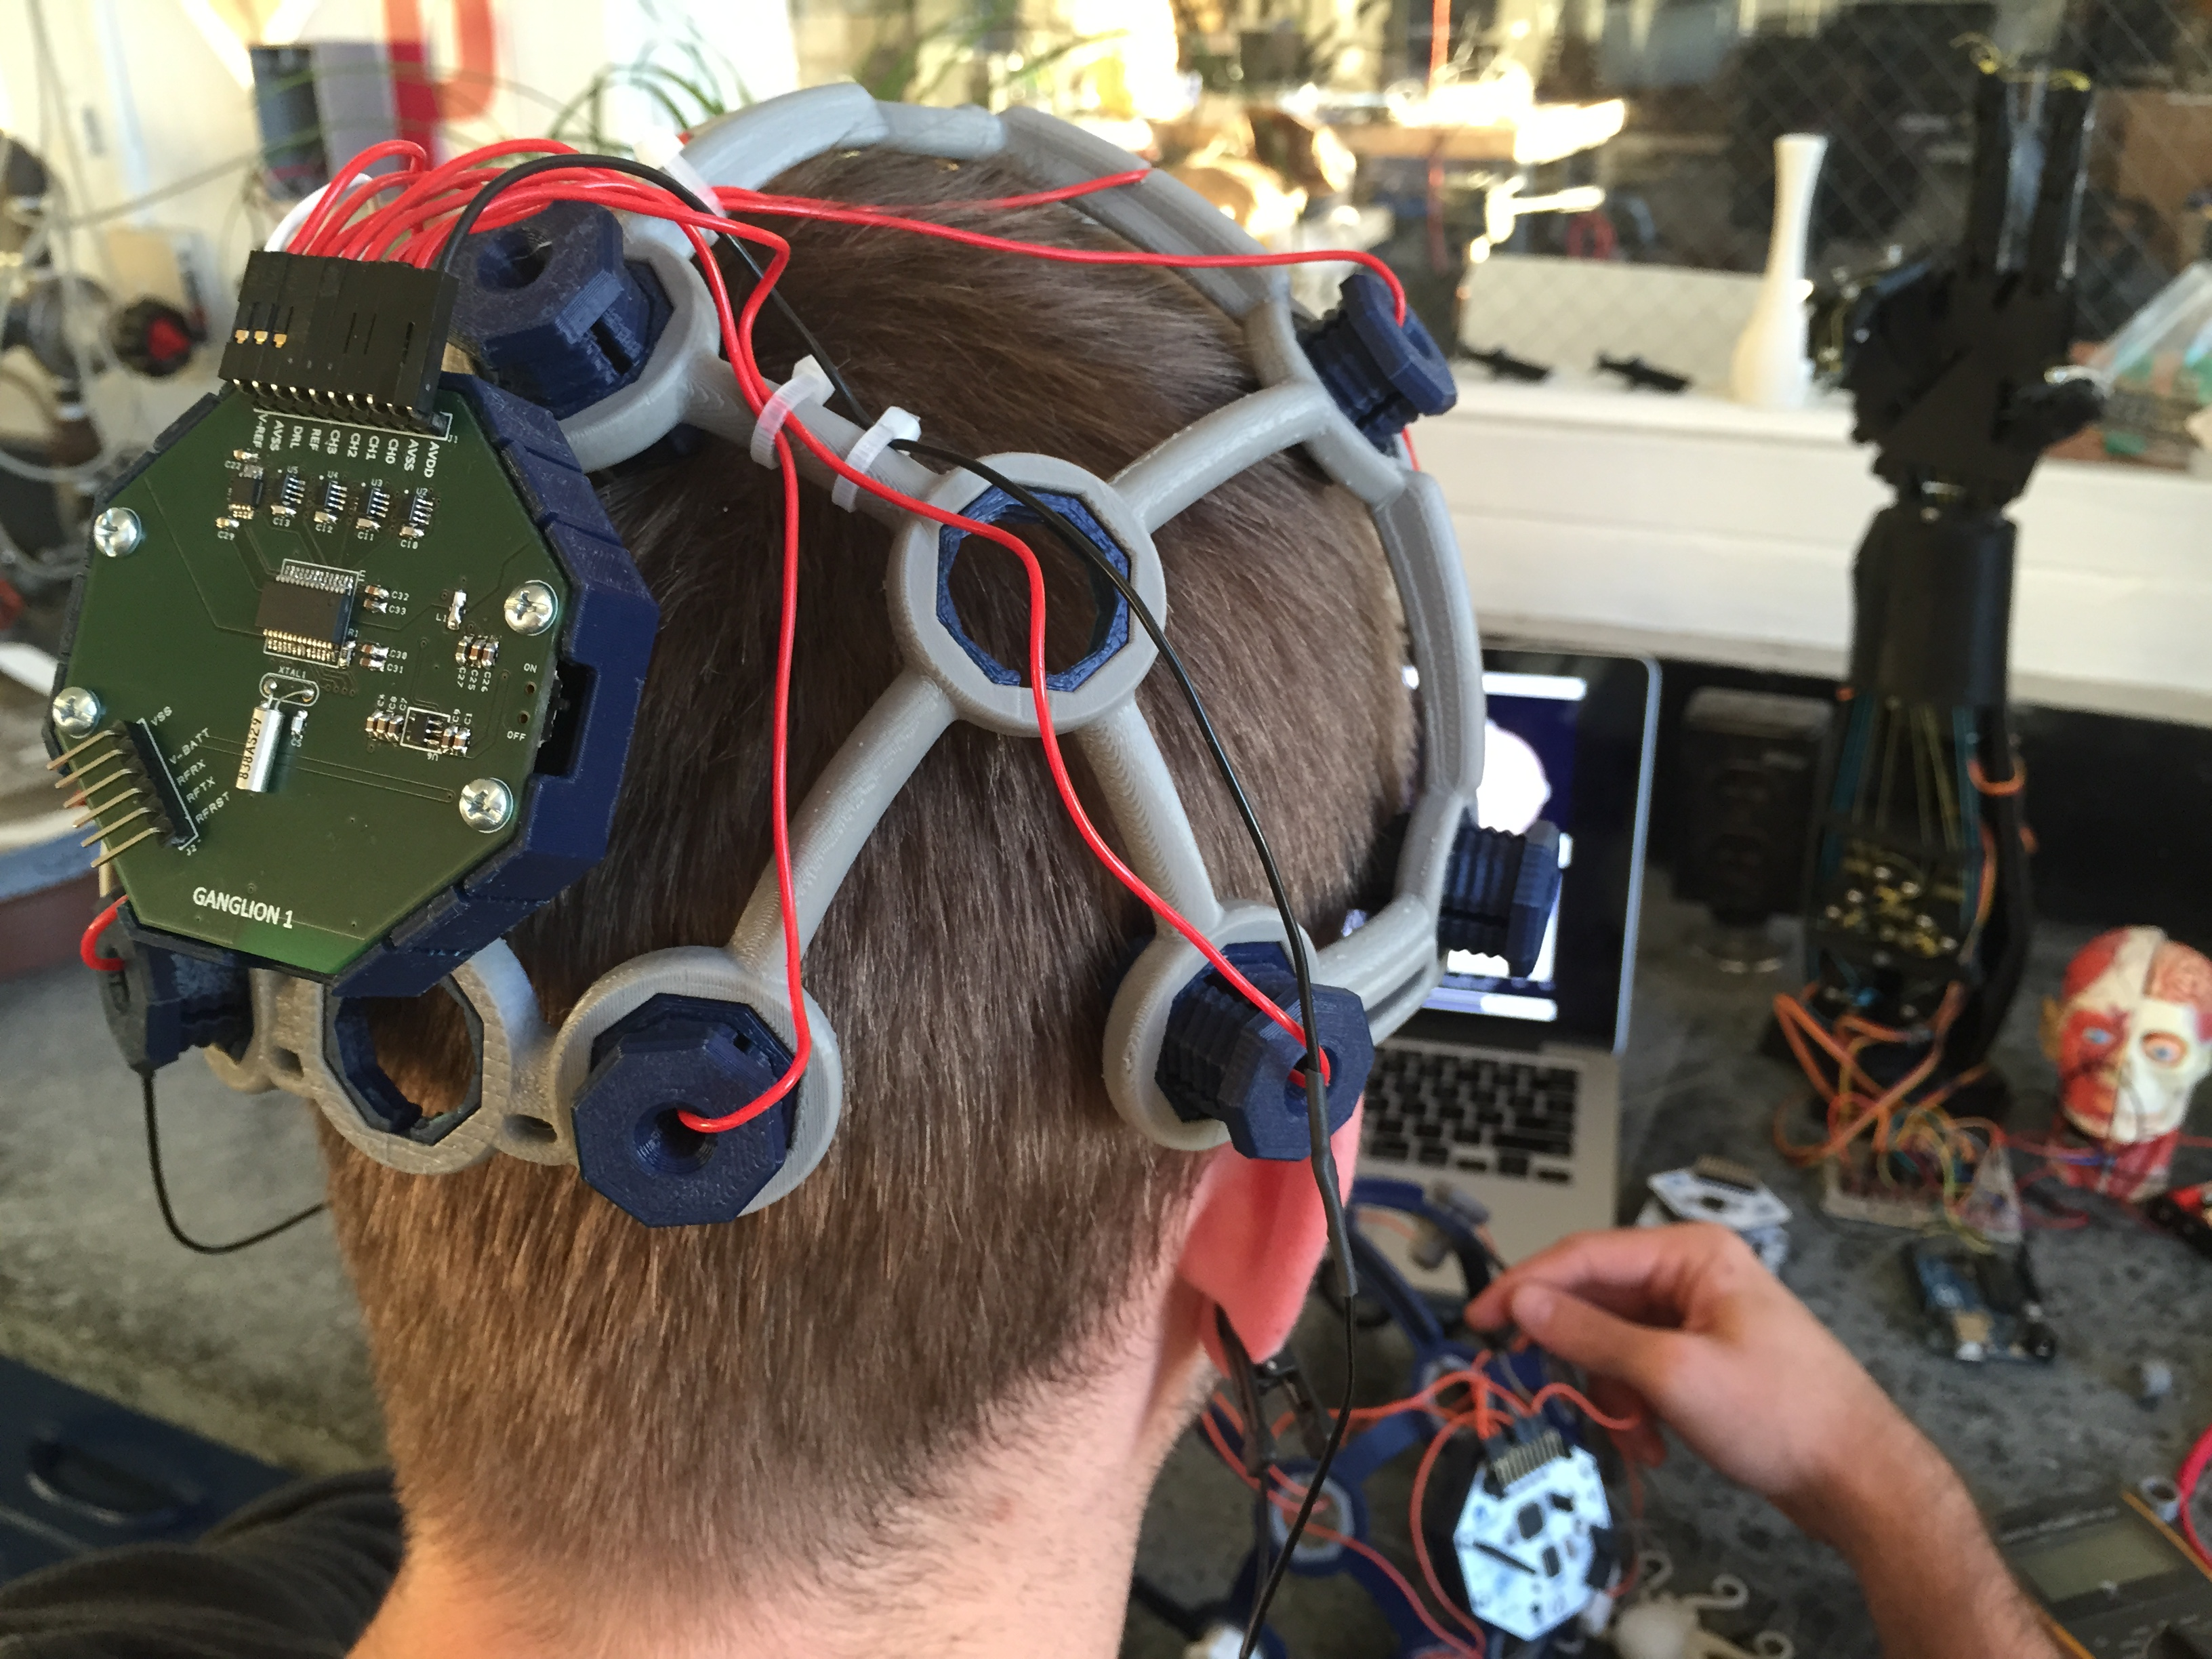
\includegraphics[width=0.8\textwidth]{files/Ultracortex-MarkIII.jpg}
  \caption{Casco impreso en 3D Ultracortex Mark III\protect\footnotemark}
  \label{fig:ultracortex}
\end{figure}
\footnotetext{\href{https://commons.wikimedia.org/w/index.php?curid=46527718}{Conorrussomanno - CC BY-SA 4.0}}

Cada uno de estos electrodos recibe el nombre de ``canal'', y permite capturar las señales eléctricas de una región del cerebro; la más próxima al electrodo. Normalmente, con mejor calidad cuanto menos pelo tenga la persona. Estas señales eléctricas son de una amplitud muy pequeña, del orden de los microvoltios.

OpenBCI registra, a una frecuencia determinada (por ejemplo, 250 Hz), la amplitud obtenida de cada uno de estos canales, y se la entrega al dispositivo al que esté conectado. Esta información también puede registrarse en un archivo, para poder acceder a ella más adelante, analizarla y filtrarla.

Estos archivos son de un tipo llamado CSV (\textit{Comma Separated Value}, valores separados por comas), en los que cada línea representa el EEG medido en un instante de tiempo. Cada línea empieza con un número, que indica el índice de la muestra concreta módulo 256, seguido de tantos \textit{samples} (medidas individuales) como canales haya. Todos los valores de una línea están, como el nombre del archivo sugiere, separados por comas.

\sombreado{¿Módulo 256?}{Si no sabe lo que significa ``módulo 256'', investíguelo. Es una operación matemática muy habitual a la hora de desarrollar algoritmos.}

A continuación tiene un archivo de una (sumamente breve) sesión de EEG creado con OpenBCI. En este caso hay 11 muestras de 4 canales (electrodos):

\begin{verbatim}
0, 214.0, -8.0, 57.0, 70.0
1, 131.0, -2.0, 60.0, 73.0
2, 79.0, 16.0, 83.0, 51.0
3, -47.0, 16.0, 55.0, 52.0
4, 83.0, -1.0, 69.0, 70.0
5, 75.0, 9.0, 69.0, 65.0
6, 168.0, 16.0, 66.0, 64.0
7, 396.0, 8.0, 69.0, 56.0
8, -53.0, -6.0, 59.0, 68.0
9, 166.0, 13.0, 57.0, 87.0
10, 228.0, 7.0, 65.0, 61.0
\end{verbatim}

\sombreado{Formato de los datos}{En esta práctica tendrá que procesar y crear ficheros con un tipo de formato (OpenBCI) y para unos datos (EEG) concretos. Este tipo de trabajo es muy habitual en la ingeniería biomédica. De hecho, todos los dispositivos biomédicos deben, de una forma u otra, procesar datos, valga la redundancia, biomédicos.}

\subsection{Objetivo y descarga de la práctica}

El objetivo de la práctica es terminar de desarrollar una aplicación Java que permite visualizar, en forma de gráficas, la información registrada en archivos en formato OpenBCI de grabaciones de EEG. Además, esta aplicación también permite la generación de archivos OpenBCI sintéticos (es decir, no capturados a partir de un sujeto humano, sino generados artificialmente). Este tipo de datos sintéticos pueden ser útiles para probar módulos \textit{software}, equipos o entrenar modelos.

La práctica está disponible en GitHub, en la siguiente dirección de Internet (URI):

\href{https://github.com/rgarciacarmona/ALED-lab1}{https://github.com/rgarciacarmona/ALED-lab1}

Para poder importar el repositorio en Eclipse seleccione \textit{File $\to$ Import...} y, de entre las opciones disponibles, \textit{Git $\to$ Projects from Git $\to$ Clone URI}. A continuación le aparecerá un menú en el que tendrá que introducir la URI que aparece en el párrafo anterior (ver Figura \ref{fig:importGit}). Es posible que, si ya copió URI antes al portapapeles, esta pantalla ya le aparezca rellena.

\begin{figure}[!htbp]
  \centering
  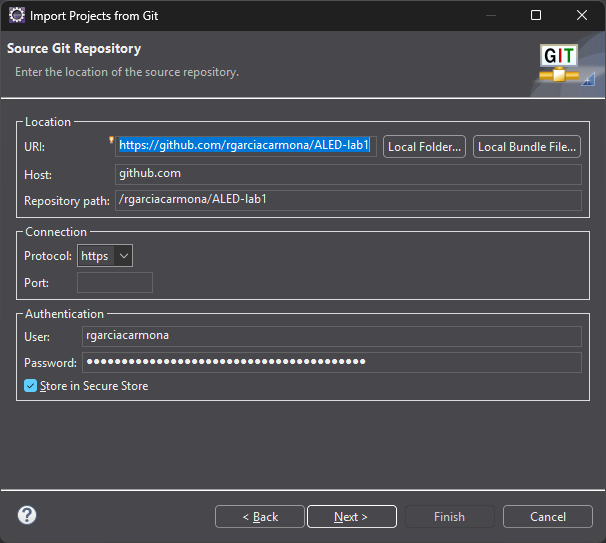
\includegraphics[width=0.8\textwidth]{files/ImportGit.png}
  \caption{Importar proyecto Git a Eclipse}
  \label{fig:importGit}
\end{figure}

Después, haga click en \textit{Next} tantas veces sea necesario y, por último, en \textit{Finish}.

A continuación, tómese su tiempo para examinar todas las clases del proyecto que acaba de importar. Intente figurarse, a base de observar el código, para qué sirve cada una de ellas. No deje de leer los comentarios; están ahí por algo.

\subsection{Modelado de datos}

Para que los datos de una sesión de EGG puedan ser manejados por un programa informático, será necesario crear un modelo de los mismos que capture toda la información relevante. Como estamos trabajando en Java, un lenguaje orientado a objetos, se han definido las siguientes clases, que deberían capturar toda la información importante presente en un archivo en formato OpenBCI: \code{EEGModel} y \code{Measurement}. Puede ver un diagrama de clases UML de las mismas en la Figura \ref{fig:uml} (no se muestran los métodos privados).

\begin{figure}[!htbp]
  \centering
  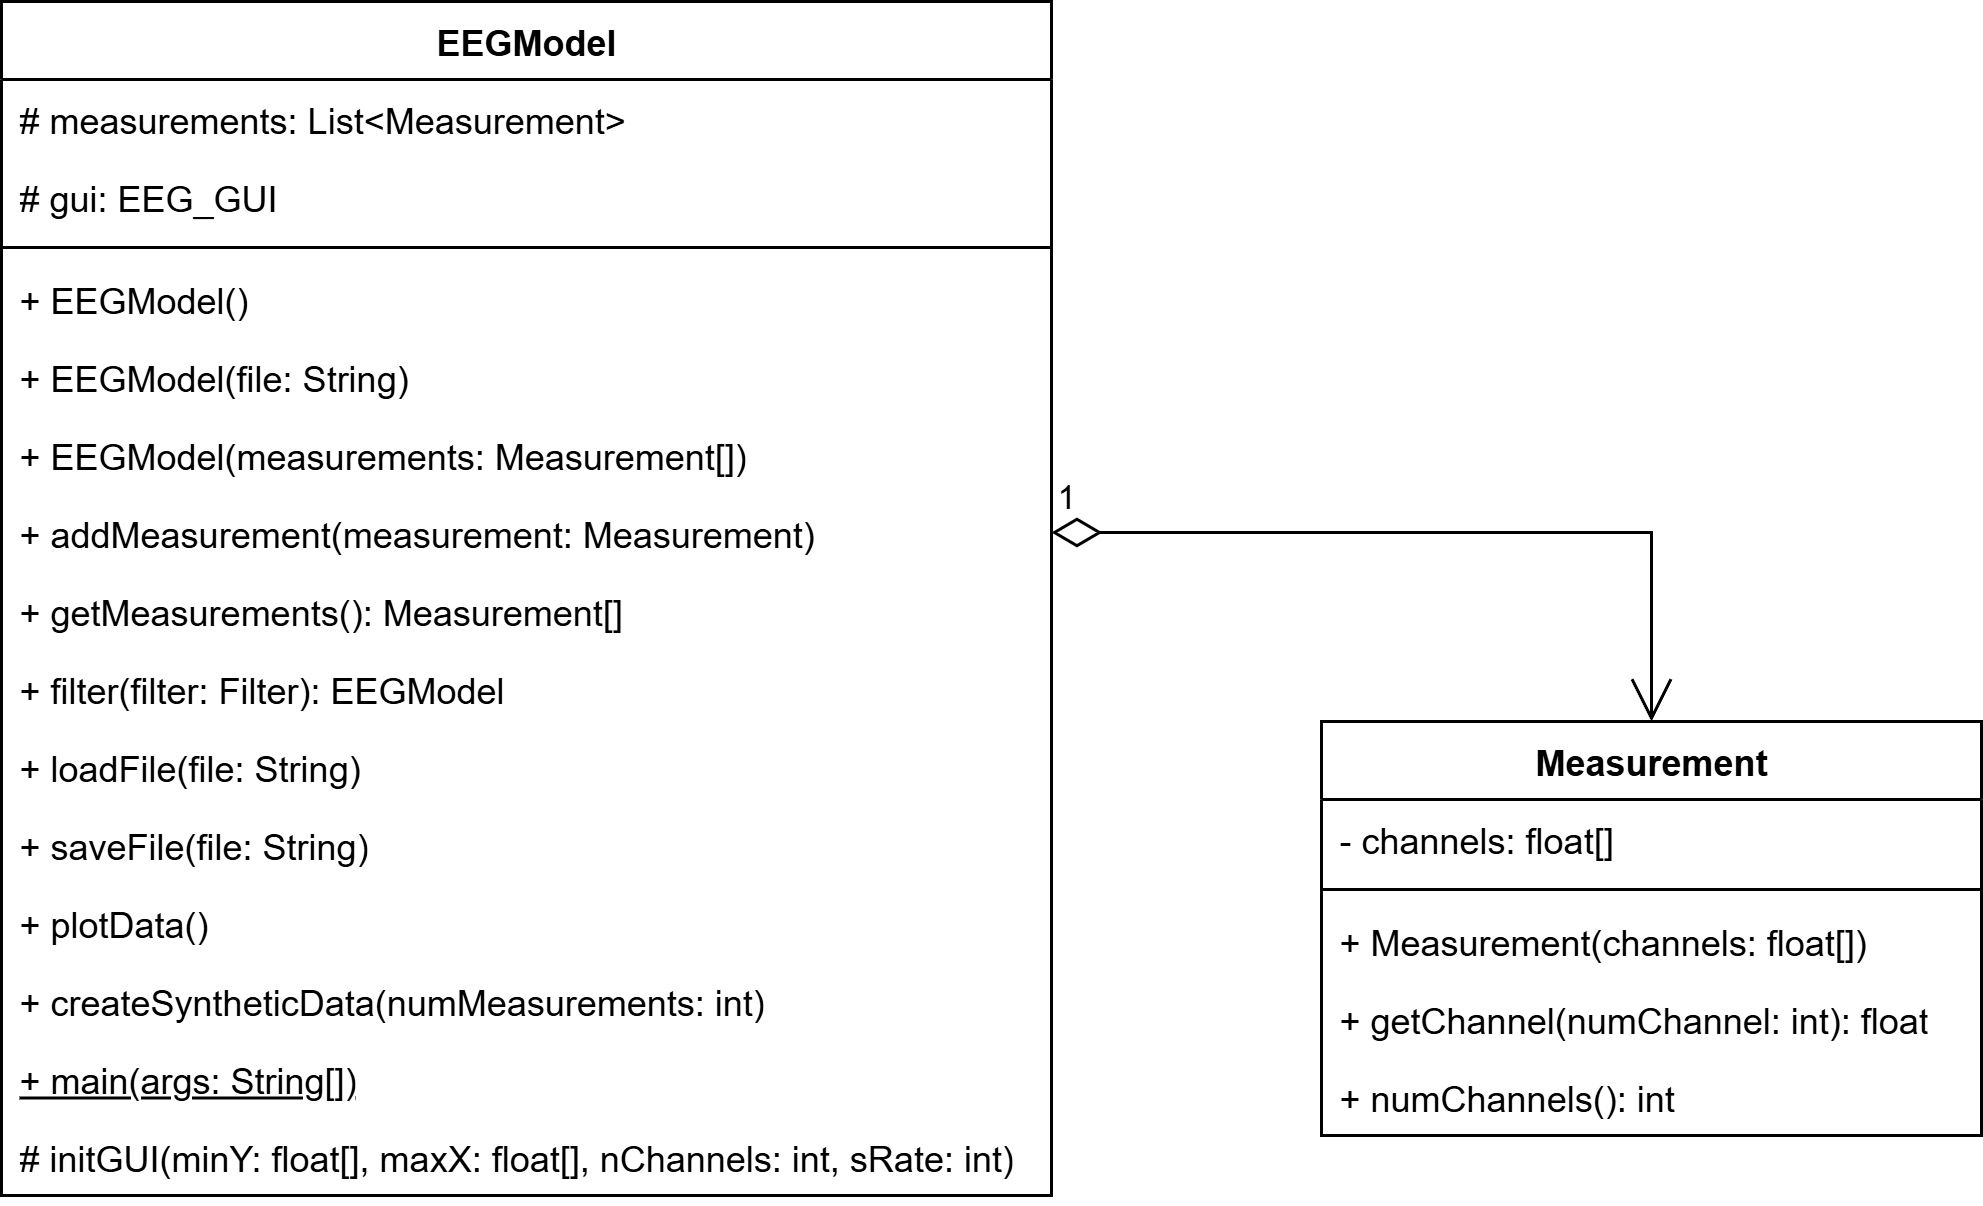
\includegraphics[width=0.8\textwidth]{files/DataModel.png}
  \caption{Diagrama de clases del modelo de datos de la práctica}
  \label{fig:uml}
\end{figure}

Intente interpretar la figura y entender cómo la información contenida en un fichero puede acabar transformada en los objetos que instancian estas dos clases. Después, abra el código fuente de ambas clases (se encuentran en el paquete \code{es.upm.aled.lab1.measurements}) y confirme que las implementaciones de los métodos hacen lo que usted sospechaba que iban a hacer tras ver el diagrama de clases.

\sombreado{// TODO}{Al examinar la clase \code{EEGModel}, habrá observado que hay una serie de métodos que contienen el comentario ``TODO''. Esto sirve para indicar aquellas partes del código que están pendientes de hacer (del inglés ``\textit{to do}''). Estas partes son, como ya habrá imaginado, las que tiene que completar para poder terminar la práctica con éxito.

Consejo: en Eclipse, se puede ver todos los \textit{TODOs} pendientes de un proyecto seleccionando la vista \textit{Window $\to$ Show View $\to$ Tasks}.}

\textbf{Responda a las siguientes preguntas:}

\begin{itemize}
    \item ¿Qué significan los símbolos ``+'', ``-'' y ``\#'' en el diagrama de clases?
    \item ¿Qué significa la flecha que conecta \code{EEGModel} con \code{Measurement} en el diagrama?
    \item Fíjese en el archivo de ejemplo de una grabación de EEG en el formato OpenBCI que aparecía en la sección \ref{eeg}. Piense en qué objetos concretos de las clases \code{EEGModel} y \code{Measurement} podrían representar este fichero. ¿De qué tamaño será la \code{List} \code{measurements} del objeto de la clase \code{EEGModel}? ¿De qué tamaño será el array \code{channels} de los objetos de la clase \code{Measurement}?
    \item ¿Cuántos métodos tiene \code{EEGModel}? ¿Cuáles aún no están implementados?
    \item ¿Cuántos argumentos puede aceptar el método \code{main} de la clase \code{EEGModel}? ¿Cuántas formas de funcionamiento tiene este método y qué hace cada una de ellas?
\end{itemize}

Enhorabuena, ya ha terminado con el trabajo previo a la sesión de laboratorio. Las secciones de la \ref{laboratorio} en adelante puede realizarlas en clase.

\subsection{Entrega de la práctica}

No es necesario entregar esta práctica ni ninguna de las siguientes. Dado que no se cuentan para la nota, ¿qué sentido tendría hacerlo? Como ya se explicó en la práctica 0, la única razón para hacer las prácticas es aprender.

La única persona que tiene que saber si ha hecho la práctica o no es usted.

\section{Guardado en archivos}
\label{laboratorio}

A continuación va a acabar de desarrollar las funcionalidades que le faltan a la aplicación para estar completa. Lo primero que hará será implementar el método \code{saveFile} de la clase \code{EEGModel}, que, como puede observar en los comentarios, debe guardar en un fichero un \code{EEGModel}; o, lo que es lo mismo, una grabación de una sesión de EEG.

En primer lugar, fíjese en la carpeta \textit{recordings}, que contiene dos archivos .txt. Ábralos y observará que ambos son archivos en el formato OpenBCI que se describió en la sección \ref{eeg}. Estos archivos son dos sesiones de EEG guardadas en el formato OpenBCI, el que aplicación deberá leer y escribir.

\textbf{Responda a las siguientes preguntas:}

\begin{itemize}
    \item ¿Cuántos canales tiene cada uno de los archivos?
    \item ¿Cuántas muestras tiene cada uno de los archivos?
\end{itemize}

\sombreado{Paquetes}{El código de la práctica se encuentra dividido en dos paquetes: uno de ellos, \code{es.upm.aled.lab1.measurements}, contiene las clases relativas al modelado y manipulado de las sesiones de EEG. El otro, \code{es.upm.aled.lab1.gui}, agrupa las clases necesarias para mostrar visualmente las gráficas de las sesiones. Este tipo de separación en paquetes es habitual en proyectos \textit{software} de cierta complejidad, y es muy útil para que nuestro cerebro no se sature con demasiada información, ocultando y apartando aquella que no es necesaria en un momento dado. En ingeniería del \textit{software}, a esto se le llama ``separación de intereses''.

La buena noticia de todo esto es que, para realizar esta práctica, solo tendrá que fijarse en las clases del paquete \textit{es.upm.aled.lab1.measurements}. El resto, en lo que a usted respecta, ``simplemente funcionan''.}

\subsection{Ejecutar el método \code{main}}

Como ya pudo observar, el método \code{main} tiene dos formas de funcionamiento:

\begin{enumerate}
    \item Recupera las muestras de una sesión de EEG almacenada en un archivo.
    \item Crea una nueva sesión de EEG sintética con muestras aleatorias.
\end{enumerate}

Cuál de las dos formas de funcionamiento se ejecuta dependerá del número de argumentos que se le pasen al \code{main}. Por defecto, al ejecutar el método \code{main} de una clase, Eclipse no le pasa ningún argumento. Por tanto, si hacemos una ejecución directa lo que hará será crear una sesión de EEG sintética.

Para pasarle parámetros al método \code{main} desde Eclipse tendremos que crear una configuración de lanzamiento. Para ello hay que hacer click-derecho en la clase que contiene el \code{main} (en nuestro caso, \code{EEGModel}), y seleccionar \textit{Run As $\to$ Run Configurations...} Esto nos llevará a una pantalla en la que podremos especificar argumentos (opción \textit{Program arguments}) e indicar desde qué carpeta va a ejecutarse la aplicación (opción \textit{Working directory}).

\begin{figure}[!htbp]
  \centering
  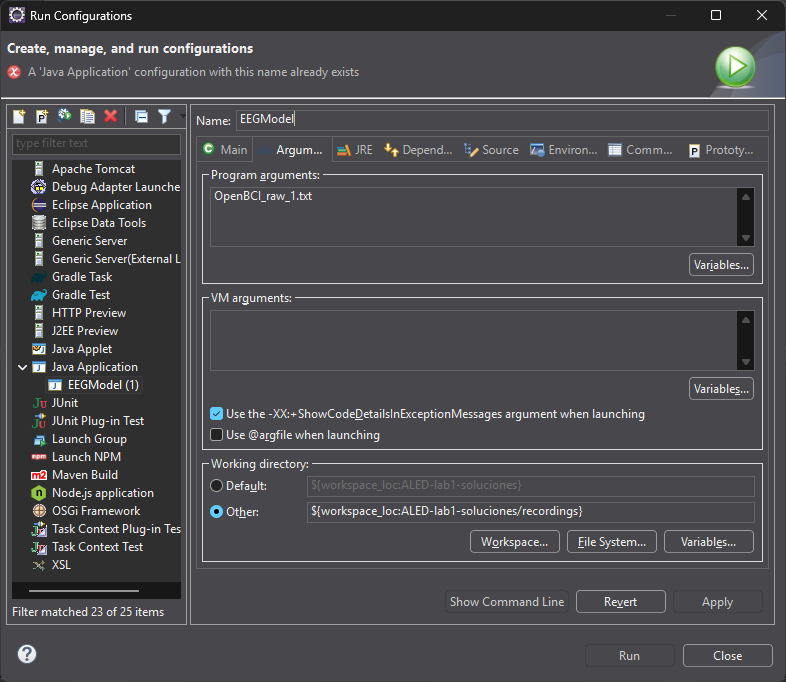
\includegraphics[width=0.8\textwidth]{files/LaunchConfiguration.png}
  \caption{Configuración de lanzamiento de ejemplo}
  \label{fig:lanzamiento}
\end{figure}

En la Figura \ref{fig:lanzamiento} puede ver cómo configurar estos parámetros para que el método \code{main} reciba como argumento el nombre de uno de los dos ficheros y se ejecute en la carpeta \textit{recordings}.

Queremos que la aplicación se ejecute en la carpeta \textit{recordings} por comodidad: cada vez que lee o escribe un fichero, la aplicación espera encontrarlo en la carpeta en la que se está ejecutando. De no ser así, hay que especificárselo manualmente (poniendo, por ejemplo \textit{recordings/OpenBCI\_raw\_1.txt} en vez de simplemente \textit{OpenBCI\_raw\_1.txt}).

A continuación, ejecute la aplicación pasándole como argumento cualquiera de los dos archivos que se encuentran en la carpeta \textit{recordings}. Tenga en cuenta que algunos canales no cambian, y que otros pueden tardar más de un minuto en experimentar cambios apreciables. Después, ejecute la aplicación de tal forma que se genere una sesión de EEG sintética.

\textbf{Responda a las siguientes preguntas:}

\begin{itemize}
    \item ¿Cuántos canales tiene la sesión sintética? ¿En qué parte del código se controla este valor?
    \item ¿Cuántas muestras tiene la sesión sintética? ¿En qué parte del código se controla este valor?
\end{itemize}

\subsection{Implementar el guardado en archivos}

Ahora debe implementar la funcionalidad necesaria para guardar una sesión (un \code{EEGModel}) en un archivo de texto siguiendo el formato CSV de OpenBCI. Es decir, el mismo formato que el método \code{loadFile} de la clase \code{EEGModel} espera encontrar. Esta funcionalidad estará contenida en el método \code{saveFile} de la clase \code{EEGModel}, por lo que deberá implementarlo.

Para ello, puede utilizar las clases \code{File}, \code{FileOutputStream} y \code{PrintStream} del paquete \code{java.io}. Recuerde que:

\begin{itemize}
    \item \code{File} le permite crear un objeto que represente un archivo a partir de su ubicación. 
    \item \code{FileOutputStream} le permite crear un \textit{stream} de salida hacia un archivo.
    \item \code{PrintStream} le permite escribir cadenas de caracteres a un \textit{stream} de salida mediante los métodos \code{print} o \code{println}. Al terminar de usar un \textit{stream}, no olvide cerrarlo. Si no, la información no quedará guardada en el archivo.
\end{itemize}

\sombreado{\code{System.out}}{Sí, \code{System.out} es un objeto de la clase \code{PrintStream}. Por eso se puede llamar a los métodos \code{print} y \code{println} sobre él.}

Después, modifique el método \code{main} para que, al terminar de generar una sesión sintética la guarde en un archivo \textit{Synthetic.txt}.

Tenga en cuenta que Eclipse tiene la mala costumbre de no actualizar automáticamente la vista del explorador de proyecto cuando se crean archivos nuevos, por lo que es posible que no vea el archivo que acaba de guardar. Para forzar este refresco en una carpeta, haga click-derecho en ella y seleccione la opción \textit{Refresh}.

\section{Filtrado de muestras}

Muchas veces los análisis de EEG se centran en partes específicas del cerebro. Las variaciones de algunos canales (la actividad de esa zona del cerebro) no son significativas y pueden ser ignoradas. Y, en otros casos, solo algunos momentos (intervalos de muestras concretos) del EEG son interesantes para el estudio que se está llevando a cabo. Por ejemplo, podríamos analizar las variaciones del EEG cuando un paciente está hiperventilando y observar solo unos canales concretos.

De hecho, al visualizar el contenido de los dos archivos de la carpeta \textit{recordings} probablemente se haya percatado usted mismo de este fenómeno; hay mucha información ``inútil''. Además, la obtención de datos en las señales biomédicas es un proceso complejo, ya que la ubicación de los sensores en el cuerpo humano es un proceso difícil y las magnitures a medir son muy pequeñas.

Para solucionar este problema, va a implementar dos filtros que permitan extraer los valores que más nos interesen de una grabación.

La aplicación proporciona un interfaz llamado \code{Filter} (ver Figura \ref{fig:filters}), que representa los métodos que cualquier filtro que deseemos crear debe implementar. En este caso estamos hablando de un único método: \code{applyFilter}. Este método acepta como argumento un \code{EEGModel} y devuelve otro \code{EEGModel} sobre el cual se ha aplicado el filtro en cuestión.

\begin{figure}[!htbp]
  \centering
  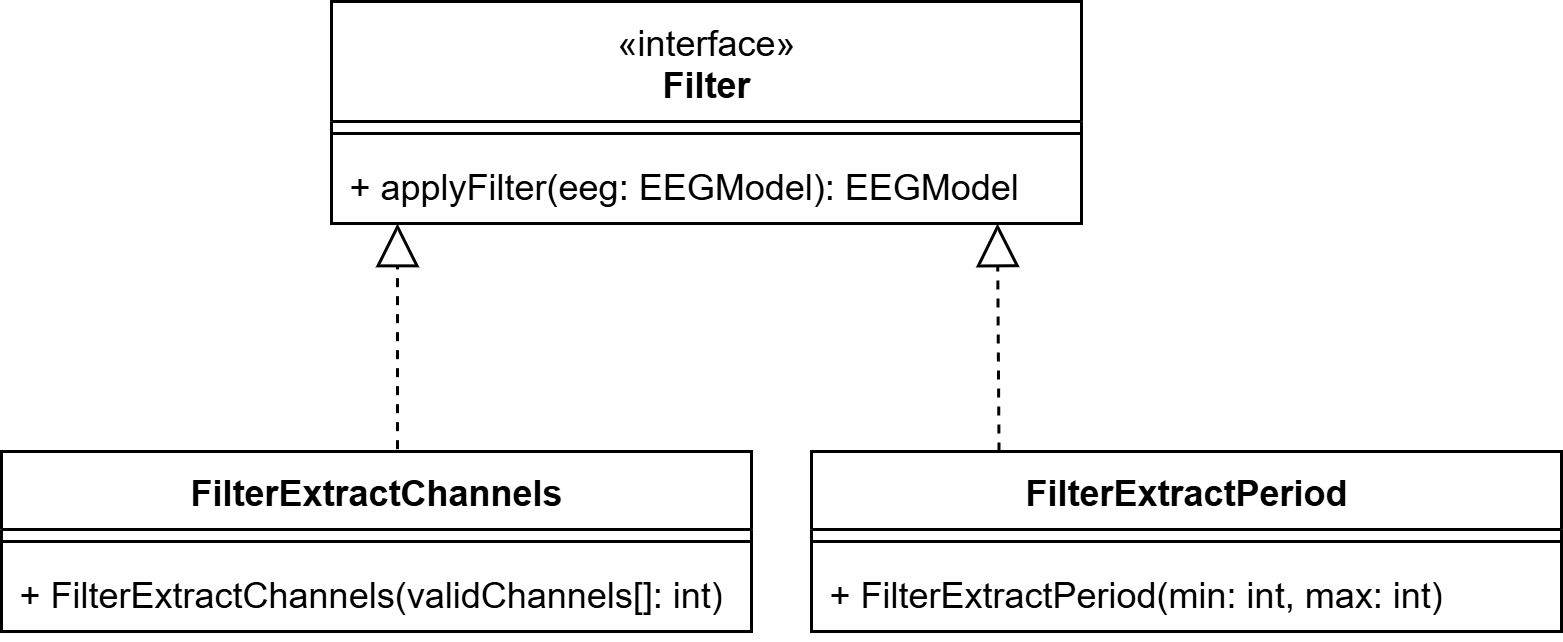
\includegraphics[width=0.8\textwidth]{files/Filters.png}
  \caption{Diagrama de clases de los filtros}
  \label{fig:filters}
\end{figure}

Deberá programar dos tipos de filtros diferentes, mediante dos clases que implementan
el interfaz \code{Filter}:

\begin{itemize}
    \item \textbf{FilterExtractChannels:} este filtro genera un nuevo \code{EEGModel} que solo incluye los canales que se pasan como argumento a su constructor. Así, si el array \code{validChannels} que se pasa como argumento contiene, por ejemplo, los enteros 3, 6 y 8, el filtro creará un nuevo \code{EEGModel} con tres canales, que corresponderán a los números 3, 6 y 8 del \code{EEGModel} sobre el que se ejecuta el método \code{applyFilter}. En este ejemplo, los tres canales del nuevo \code{EEGModel} serán los números 0, 1 y 2; y se corresponderán con los canales 3, 6 y 8, respectivamente, del \code{EEGModel} original.
    \item \textbf{FilterExtractPeriod:} este filtro extraerá un intervalo de muestras concreto, que viene delimitado por los dos enteros (\code{min} y \code{max}) que se pasan como parámetros al constructor: \code{min} será el índice de la primera muestra seleccionada y \code{max} el de la última muestra seleccionada. Los dos límites deben estar incluidos en el rango. Si, por ejemplo, los argumentos \code{min} y \code{max} son 501 y 750, el filtro creará un nuevo \code{EEGModel} con estas 250 muestras del \code{EEGModel} original.
\end{itemize}

Para implementar ambos filtros probablemente necesite implementar también el constructor de \code{EEGModel} que acepta como argumento un array de \code{Measurements}. Así que no olvide hacerlo.

Por último, implemente el método \code{filter} de \code{EEGModel} que permite aplicar un filtro sobre sí mismo.

Para comprobar que el código que ha programado funciona, modifique el método \code{main} para que lea el contenido del archivo \textit{OpenBCI\_raw\_1.txt} y, usando el método \code{filter}, extraiga solo los 3 últimos canales y las muestras desde la 2750 y 5750 ,y las dibuje en pantalla. Observará cómo ahora sí que estamos visualizando información relevante.

Enhorabuena, ha terminado la práctica.

\section{Extras}

Si siente curiosidad, pruebe a llevar a cabo las tareas siguientes:

\begin{itemize}
\item Dibuje un diagrama de clases completo del proyecto.
\item Investigue cómo funcionan las clases del paquete \code{es.upm.aled.lab1.gui}.
\item Cree un tercer filtro, que tenga dos parámetros en su constructor: un canal (\code{int}) y un umbral (\code{float}). Este filtro deberá encontrará la primera muestra cuya medida (\textit{sample}) en el canal especificado supere el umbral, y creará un nuevo \code{EEGModel} que contenga solo las 100 muestras anteriores, la muestra encontrada, y las 100 muestras siguientes.
\end{itemize}

\end{document}